\section{路径规划与车道保持算法}

\subsection{强化学习与神经网络概述}
强化学习的历史可以用两条各自独立但丰富多彩的主线来追溯。。一条主线聚焦于研究最优化控制,以及使用价
值函数动态规划等算法来寻找问题的解决方案。另一条主线源于研究动物学习心理学时产生的试错学习,对它的研究也诞生了早期 人工智能的其他领域,其一直是强化学习的主要研究内容。这两条主线在很长时间里是相对独立发展的,如今的强化学习理论主要是第二条主线的延续。如今的
强化学习主要研究这样一类问题:具有一定思考和行为能力的个体(Agent)在与其所处的环境(Environment)进行交互的过程中,
通过学习策略达到奖励最大化或实现特定的目标。其中,“个体”处在“环境”中,在某时刻可以有一个对自身的认识,这可以表示成个体自身在该时刻的状态(State)。
个体在某时刻可以向环境实施一个行为(Action),环境会因为这一行为做出相应的改变并给予个体一定形式的反馈,
个体接收到这个反馈后可以建立“自身状态”“所施行为”及“所得反馈”之间的联系,作为自身记忆的一部分给后续的决策提供参考。
个体在不同状态下向环境施加的各种不同行为则构成了个体与环境交互的“策略”(Policy)。个体策略的构建与个体的目的密切相关。
环境给予个体一个表征当前环境对个体奖惩程度的数值,我们一般称之为“奖励”(Reward)。
个体构建策略的目的就是要争取通过与环境的交互而获得尽可能多的累积奖励值。强化学习过程可用~\ref{fig:3_1}来说明。
\begin{figure}[H]
  \centering
  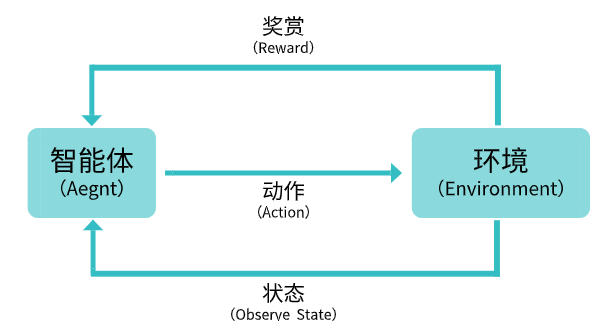
\includegraphics[width=0.5\linewidth]{fig/rl.png}
  \caption{\textbf{强化学习过程}}
  \label{fig:3_1}
\end{figure}

强化学习包括有模型强化学习和免模型强化学习,本章均会介绍。强化学习过程满足马尔科夫性。一般我们把强化学习认为是一个马尔科夫决策过程 。强化学习因为要与环境进行交互,所以会有探索与利用问题,
本章也介绍了此问题的一般解决算法即使用$\epsilon$-贪心策略来解决。
\subsubsection{$\epsilon$-贪心策略}
强化学习通过与环境的交互来累计奖励,但当agent在环境中时,就会陷入一个被称为探索利用困境的局面。
即agent如果只考虑当前奖励最大化,不去探索环境可能会错失最优解。下面通过“K-摇臂赌博机”(K-armed bandit)
问题来详细说明一下。K-摇臂赌博机(图~\ref{fig:3_2})是一种博弈类游戏工具,一台机器上有多个拉杆。赌徒拉下一个拉杆后,游戏机会随机给予一定数额的奖励。赌徒
一次只能拉下一个拉杆,每个拉杆的奖励分布是彼此独立的,即后一次拉杆奖励与前一次无关。在这个场景中,游戏机相当于环境。
个体拉下某一单臂游戏机的拉杆表示执行了一个特定的行为,游戏机会给出一个即时奖励R,随即该状态序结束。赌徒的目标是通过一定的策略
使自己获得的奖励最大化。若赌徒采取仅探索策略,即将所有机会平均分给每个摇臂,多次试验后得到每个摇臂奖励的期望,之后仅选择期望最大的摇臂。
若采用仅利用策略,即按下目前最优的(目前为止奖励最大的摇臂)摇臂。显然,“仅探索”发在估计途中,丧失了许多得到最大奖励的机会,但它较好的估算了每个摇臂的奖励
;“仅利用”发相反,它没有对摇臂奖励进行估计,选择的摇臂往往不是最优的。综上,两种方法都很难使人满意,要想达到令人满意的成果就要把二者结合起来,即在探索和利用
之间进行折中。
\begin{figure}[H]
  \centering
  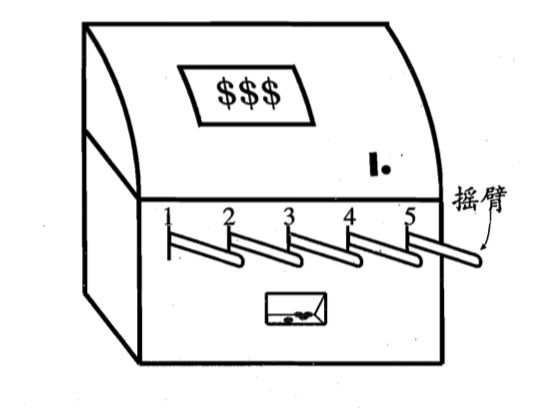
\includegraphics[width=0.6\linewidth]{fig/kab.jpg}
  \caption{\textbf{K-摇臂赌博机}}
  \label{fig:3_2}
\end{figure}

$\epsilon$-贪心策略使用一个浮动的概率来对探索和利用进行折中:每次迭代时
以$\epsilon$的概率进行探索,即以随机选择动作;以1-$\epsilon$的机率进行利用,即选择当前奖励值
最高的动作。实际程序中$\epsilon$常是一个变化的值,即在开始是$\epsilon$较大,随着与环境 交互轮数的
提升$\epsilon$越来越小。本文所用$\epsilon $贪心策略算法1所示。可以看到本文所用的$\epsilon $贪心策略是浮动变化的,开始时为一个较大的值$\epsilon_s$,最后接近于一个趋于0的值$\epsilon_e$,这样做可以很好地平衡探索与利用之间的矛盾。
\begin{algorithm}[H] 
  \caption{$\epsilon$-贪心策略}  
  \begin{algorithmic}[1] 
    \Require 起始$\epsilon$值 $\epsilon_s$ ; 终止$\epsilon$值 $\epsilon_e$ ; 
    尝试次数 T; 衰减因子 $\epsilon_d$
    \Ensure  
    \For {each $i \in T$}
      \If {$i\%Decay_{cycle}==0$}
      \State $\epsilon_d$=$\epsilon_d\times0.8$
      \EndIf
      \If {$rand()<\epsilon $}
      \State $k=from 1,2,......,K$中以均匀分布随机选取
      \Else
      \State $k=argmax_{i}Q(i)$
      \EndIf
      \State $\epsilon = \epsilon_e+(\epsilon_s- \epsilon_e)e^{\frac{-i}{\epsilon_d }}$
    \EndFor   
  \end{algorithmic}  
\end{algorithm}

\subsubsection{马尔科夫决策过程}
在一个时序过程中,如果$t+1$时的状态仅依赖于$t$时的状态$S_t$,而与$t$时之前的任何状态都无关,就定义$t$时的状态$S_t$具有马尔可夫性质(Markov Property,简称MP)。
若过程中的每一个状态均满足上述MP,则这个过程就具备MP。具备了此性质的随机过程称为马氏过程(Markov Process),简称MP
或习惯性称为马氏链(Markov Chain,简称MC)。MC可以由一个元组$<S,P>$来描述。其中$S$是有限状态集合,$P$是状态转移概率矩阵
MP的每一个状态$S_t$都仅依赖于上一个状态即状态具有完备性,而且一旦$S_t$确定了,历史状态信息$S_1,S_2,…,S_{t-1}$对于确定$S_{t+1}$就不再重要,可有可无。
用数学描述为
\begin{equation}
  P[s_{t+1}|s_t]=P[s_{t+1}|s_1,....s_t]
  \label{eq:3-1}
\end{equation}
如果一个决策过程满足MP,我们就定义这个决策过程为马尔科夫决策过程(Markov Decision Process,简称 MDP)。
至此,我们用一个$<S,A,P,R,\gamma >$来描述
一个MDP,其中$S$为有限状态集合,$A$为有限动作集合,$P$为状态转移概率矩阵,$R$为奖励函数,$\gamma $是计算累计回报时的
奖励因子。一般的MDP都对应一个策略$\pi$ ,给定策略下的累计回报如 式\eqref{eq:3-2}
\begin{equation}
  G_t=R_{t+1}+\gamma R_{t+2}+...=\sum_{k = 0}^{\infty} \gamma ^kR_{t+k+1} 
  \label{eq:3-2}
\end{equation}
我们定义在MDP中使用状态价值函数来衡量一个状态的价值,策略$\pi$下的状态
价值函数如 式\eqref{eq:3-3}
\begin{equation}
  v_\pi (s)=E_\pi [\sum_{k = 0}^{\infty}\gamma ^kR_{t+k+1}|S_t=s ]
  \label{eq:3-3}
\end{equation}
进而考虑每个动作的价值,定义动作价值函数如式 \eqref{eq:3-4}
\begin{equation}
  q_\pi (s,a)=E_\pi [\sum_{k = 0}^{\infty}\gamma ^kR_{t+k+1}|S_t=s,A_t=a ]
  \label{eq:3-4}
\end{equation}
根据MDP过程的马尔科夫性质,我们可以将式\eqref{eq:3-3}、\eqref{eq:3-4}改写为Bellman方程:
\begin{equation}
  v_\pi (s)=E_\pi [\sum_{k = 0}^{\infty}\gamma ^kR_{t+k+1}|S_t=s ]
  =E_\pi [R_{t+1}+\gamma v(S_{t+1})|S_t=s]
  \label{eq:3-5}
\end{equation}
\begin{equation}
  q_\pi (s,a)=E_\pi [\sum_{k = 0}^{\infty}\gamma ^kR_{t+k+1}|S_t=s,A_t=a ]
  =E_\pi [R_{t+1}+\gamma q(S_{t+1},A_{t+1})|S_t=s,A_t=a]
  \label{eq:3-6}
\end{equation}
给定策略$\pi $下的MDP问题可以通过其衍生的MRP(Markov Reward Process)和转移矩阵$P$来求解。由上式可知不同的策略可以得到不同的价值函数,这些价值函数之间的具有一定的不同。那么是否存在一个基于某一策略的价值函数,
在该策略下每一个状态的价值都高于其他策略?如果存在,如何找到这样的价值函数?这样的价值函数对应的策略又是什么?为了回答这些问题
,我们需要引入下述几个最优函数概念,它们之间相互对应,这也是Bellman最优递归方程的原理。

定义最优价值函数$v^*(s)$如式\eqref{eq:3-7}。最优动作值函数$q^*(s,a)$
如式\eqref{eq:3-8},即:
\begin{equation}
  v^*(s)=\max\limits_{\pi} v_\pi(s)
  \label{eq:3-7}
\end{equation}
\begin{equation}
  q^*(s,a)=\max\limits_{\pi} q_\pi(s,a)
  \label{eq:3-8}
\end{equation}
由式\eqref{eq:3-7}、\eqref{eq:3-8}可得$v^*(s)$函数和$q^*(s,a)$函数的Bellman方程
,其中$s^{'},a^{'}$分别代表下一时刻的动作和状态:
\begin{equation}
  v^*(s)=\max\limits_{a}R_s^a+\gamma \sum_{s^{'}\in{S}}P_{ss_{'}}^av^*(s^{'}) 
  \label{eq:3-9}
\end{equation}
\begin{equation}
  q^*(s,a)=R_s^a+\gamma \sum_{s^{'}\in{S}}P_{ss_{'}}^a\max\limits_{a}q^*(s^{'},a^{'}) 
  \label{eq:3-10}
\end{equation}
若已知$q^*(s,a)$,最优策略可以通过直接最大化$q^*(s,a)$来求出:
\begin{equation}
 \pi ^*(s,a)=\left\{
\begin{array}{rcl}
1       &      & {if(a=arg\max\limits_{a\in{A}} q^*(s,a))}\\
0     &      & {otherwise}\\


\end{array} \right. 
\label{eq:3-11}
\end{equation}
至此,MDP相关内容介绍完毕,其实根据Bellman最优方程可以得出最优策略,但由于Bellman最优
方程不是线性的,求解其的空间复杂度为$O(n^3)$,对于正常规模的强化学习问题无法直接求解,
且强化学习问题的环境$P$概率转移矩阵并非都是已知的,甚至大多数情况下其都是未知的。
下面就将介绍免模型学习的经典算法蒙特卡罗强化学习\upcite{r20},简称MCRL。
\subsubsection{蒙特卡罗强化学习}
在求解无模型强化学习问题 中,$P_{ss_{'}}^a$是未知的,已知的只有每一步动作的奖励以及下一个状态
。受到上文探索与利用问题的启发,可以利用一个周期内的智能体状态奖励数据,通过求取采样数据的期望来求解动作值函数,以解决环境未知带来的问题。这种方法被称为蒙特卡洛强化学习。
从下面的伪代码可以看出被评估和改进的算法都是同一个策略,因此称为同策略MC算法。
\\
\begin{algorithm}[H]  
  \caption{同策略MC法}  
  \begin{algorithmic}[1] 
    \Require 环境 E ; 动作空间 A ;
    策略执行步数 T ; 起始状态 $x_0$;
    \Ensure 
    \State $Q(s,a)=0,count(x,a)=0,\pi(x,a)=\frac{1}{|A(x)|} $ 
    \For{each $s \in T$}
    \State 在E中执行策略$\pi $产生轨迹
    \State $<x_0,a_0,r_1,a_1,r_2,.....,x_{T-1},r_T,x_T>;$
    \For{}
    \State$R=\frac{1}{T-t} \sum_{i=t+1}^{T}r_i ; $
    \State$Q(x_t,a_t)=\frac{Q(x_i,a_t)\times{count(x_t,a_t)}+R}{count(x_t,a_t)+1};$
    \State$count(x_t,a_t)=count(x_t,a_t)+1$
    \EndFor
    \State 对所有已见状态x:
    \State$$
    \pi (x)=\begin{cases}
      a=arg\max\limits_{a\in{A}} q^*(s,a)& \text{以概率1-$\epsilon$  }\\
      \text{以均匀概率从A中选取动作}& \text{以概率$\epsilon$ }
    \end{cases}
    $$
    \EndFor   
  \end{algorithmic}  
\end{algorithm}

\subsubsection{深度学习与神经网络}
深度学习(Deep Learning,简称DL)即神经网络,其通过人工神经元的相互连接让机器学会表示本身,即通过其他简单的
表示来表达复杂的表示,解决了表示学习中的核心问题。如今的人工智能浪潮,可以说就是因为深度学习的成功应用引起的。深度学习通过非线性激活函数以及隐藏层的作用,可以模拟任何函数及其导数,利用此特点,本文利用神经网络近似Q学习的值函数,下面介绍两种常见的神经网络。
\subsubsection{全连接神经网络}
全连接神经网络属于深度前馈网络的一种,下文的卷积神经网络也是深度前馈网络。全连接神经网络结构如图~\ref{fig:3-3}所示。神经网络能够拟合非线性函数的原因在于,每个神经元的非线性激活函数,常用的激活函数有sigmoid、Tanh、Relu等。本文所用激活函数
为Relu激活函数。
\begin{figure}[H]
  \centering
  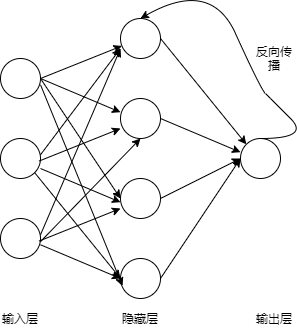
\includegraphics[width=7cm,height=7cm]{fig/mlp.png}
  \caption{\textbf{全连接神经网络}}
  \label{fig:3-3}
\end{figure}

\subsubsection{卷积神经网络}
卷积神经网络(Convolutional Neural Networks,简称 CNN),是一种使用了卷积运算的神经网络,利用卷积运算的性质,其可以很好的提取诸如图像这类矩阵类型的数据
。CNN可以说是最成功的神经网络之一,其结构如图~\ref{fig:3-4}所示。
\begin{figure}[H]
  \centering
  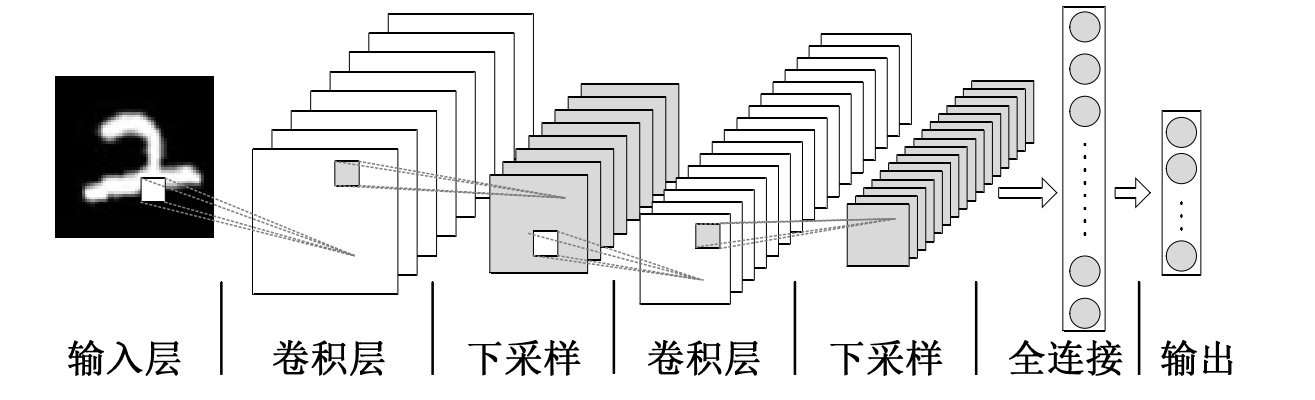
\includegraphics[width=0.9\linewidth]{fig/cnn1.png}
  \caption{\textbf{卷积神经网络}}
  \label{fig:3-4}
\end{figure}

\subsection{路径规划强化学习算法}
MC算法利用一个周期内的智能体状态奖励数据,通过求取采样数据的期望来求解动作值函数,以解决环境未知带来的问题。其缺点是运行效率较低。导致其的主要原因是MC算法没有很好地利用MDP的性质。
时序差分(Temporal-Difference Reinforcement Learning,简称TD学习)强化学习
结合了动态规划法和MC法,可以实现更高效的免模型学习,下面分别介绍同策略的TD学习(SARSA)和异策略的TD学习(Q
learning),SARSA是一个同策略算法,因为伪代码中评估(第六行),执行(第五行)的均为$\epsilon$贪心策略。
Qlearning则是异策略算法,伪代码中评估(第六行)的是原始策略,执行(第四行)的是$\epsilon$
贪心策略。本文所用的强化学习路径规划方法即这两个算法迁移到路径规划中来,并对奖励函数进行了定制处理,以满足用户需要,因为
两个算法的相似性,下面仅列出Q学习路径规划的代码。

可以看到使用Q学习进行路径规划即通过与环境交互得到当前环境下使得累计奖励最大的Q函数,通过最大化Q值函数选取路径点。Q学习的核心为其算法的更新公式即
\begin{equation}
  Q(s,a)=Q(s,a)+\alpha (r+\gamma Q(x^{'},a{'})-Q(x,a))
  \label{eq:3-12}
\end{equation}
其中$x^{'}$是前一次在状态$x$执行动作$a$转移到的状态,$a^{'}$是策略$\pi$在$x^{'}$上选择的动作;$\alpha$为学习率,其值越大
Q值收敛越快,但很可能会导致路径规划效果较差;$\gamma$为折扣因子,表示智能体的“远见程度”。$r$是指智能体执行动作$a$后所获得的奖励,
可以通过个性化设计来满足不同人的需求,可以说奖励函数的设计是强化学习任务的核心,本文的奖励函数即采用作者喜好的奖励函数,即将距离远近作为第一考虑要素。
根据Q学习更新公式,可以证明,在学习率满足0-1之间,Q学习可以
保证在无模型条件下收敛\upcite{r19}。\\
\begin{algorithm}[H]  
  \caption{SARSA}  
  \begin{algorithmic}[1] 
    \Require 环境 E ; 动作空间 A ;
     起始状态 $x_0$;折扣奖励$\gamma $;更新步长$\alpha $;
    \Ensure 
    \State $Q(s,a)=0,\pi(x,a)=\frac{1}{|A(x)|} $ ;
    \State $x=x_0,a=\pi(x);$
    \For{each $t=1,2,....do $}
    \State $r,x^{'}$=在E中执行动作a产生的奖励和转移的状态;
    \State $a^{'}=\pi^{\epsilon }(x^{'})$
    \State $Q(s,a)=Q(s,a)+\alpha (r+\gamma Q(x^{'},a{'})-Q(x,a));$
    \State $\pi(x)=arg\max_{a^{''}}Q(x,a^{''});$
    \State $x=x^{'},a=a^{'}$
    \EndFor   
  \end{algorithmic}  
\end{algorithm}

\begin{algorithm}[H]  
  \caption{Qlearning}  
  \begin{algorithmic}[1] 
    \Require 环境 E ; 动作空间 A ;
     起始状态 $x_0$;折扣奖励$\gamma $;更新步长$\alpha $;
    \Ensure 
    \State $Q(s,a)=0,\pi(x,a)=\frac{1}{|A(x)|} $ ;
    \State $x=x_0;$
    \For{each $t=1,2,....do $}
    \State $r,x^{'}$=在E中执行动作$a=\pi^{\epsilon}(x)$产生的奖励和转移的状态;
    \State $a^{'}=\pi(x^{'})$
    \State $Q(s,a)=Q(s,a)+\alpha (r+\gamma Q(x^{'},a{'})-Q(x,a));$
    \State $\pi(x)=arg\max_{a^{''}}Q(x,a^{''});$
    \State $x=x^{'}$
    \EndFor   
  \end{algorithmic}  
\end{algorithm}

\begin{algorithm}[H]  
  \caption{Qlearning路径规划}  
  \begin{algorithmic}[1] 
    \Require 环境 E ; 动作空间 A ;
     起始状态 $x_0$;折扣奖励$\gamma $;更新步长$\alpha $;迭代轮数 N;起始点和终点;
    \Ensure 
    \State $Q(s,a)=0,\pi(x,a)=\frac{1}{|A(x)|} $ ;
    \For{each $i=1,2,....Ndo $}
    \State $x=x_0;$初始化状态即回到起始点
    \For{each $t=1,2,....do $}
    \State $r,x^{'}$=在E中执行动作$a=\pi^{\epsilon}(x)$产生的奖励和转移的状态;
    \State $a^{'}=\pi(x^{'})$
    \State $Q(s,a)=Q(s,a)+\alpha (r+\gamma Q(x^{'},a{'})-Q(x,a));$
    \State $\pi(x)=arg\max_{a^{''}}Q(x,a^{''});$
    \State $x=x^{'}$
    \If{$x^{'}==end_{point}$即到达终点}
    \State $break$
    \EndIf
    \If{$x^{'}==obs$撞到障碍物}
    \State $break$
    \EndIf
    \EndFor
    \EndFor   
  \end{algorithmic}  
\end{algorithm}



\subsection{车道保持DQN算法}
DQN\upcite{r7}算法起源于2015年谷歌团队于nature上发表的Human-level control through deep reinforcement
learning。这篇论文中 提 出 的DeepQNetwork(DQN) 算法在
Atari游 戏 中 取得 了媲美人类职业玩家的成绩, DQN算法将深度神经网 络 应
用 到 强化学 习 算法 中 , 是深度强化学习的开山之作。其根据输入的 Atari 游戏屏 幕 图 片 , 选取一系列动作使得游戏得分最高。 下面将介绍DQN算法以及本文所用DQN算法框架。

\subsubsection{DQN算法原理}
DQN算法是在对传统的Q学习算法的改进上得来的,传统的Q学习算法,在面对大规模状态空间时,需要建立大规模的Q表即值函数,极其占用计算资源
研究人员称之为维度灾难。DeepMind团队DQN基本原理就是利用CNN的强大表达能力模拟Q值函数,如式\eqref{eq:3-13}
\begin{equation}
  f(s,a,w)\approx Q^*(s,a)
  \label{eq:3-13}
\end{equation}
GooleDeepMind团队DQN网络示意图如图~\ref{fig:3-5}所示,可以看到,DQN算法使用游戏屏幕图像作为输入经过
CNN的特征提取和动作输出,在Atari游戏上取得了不错的表现。
\begin{figure}[H]
  \centering
  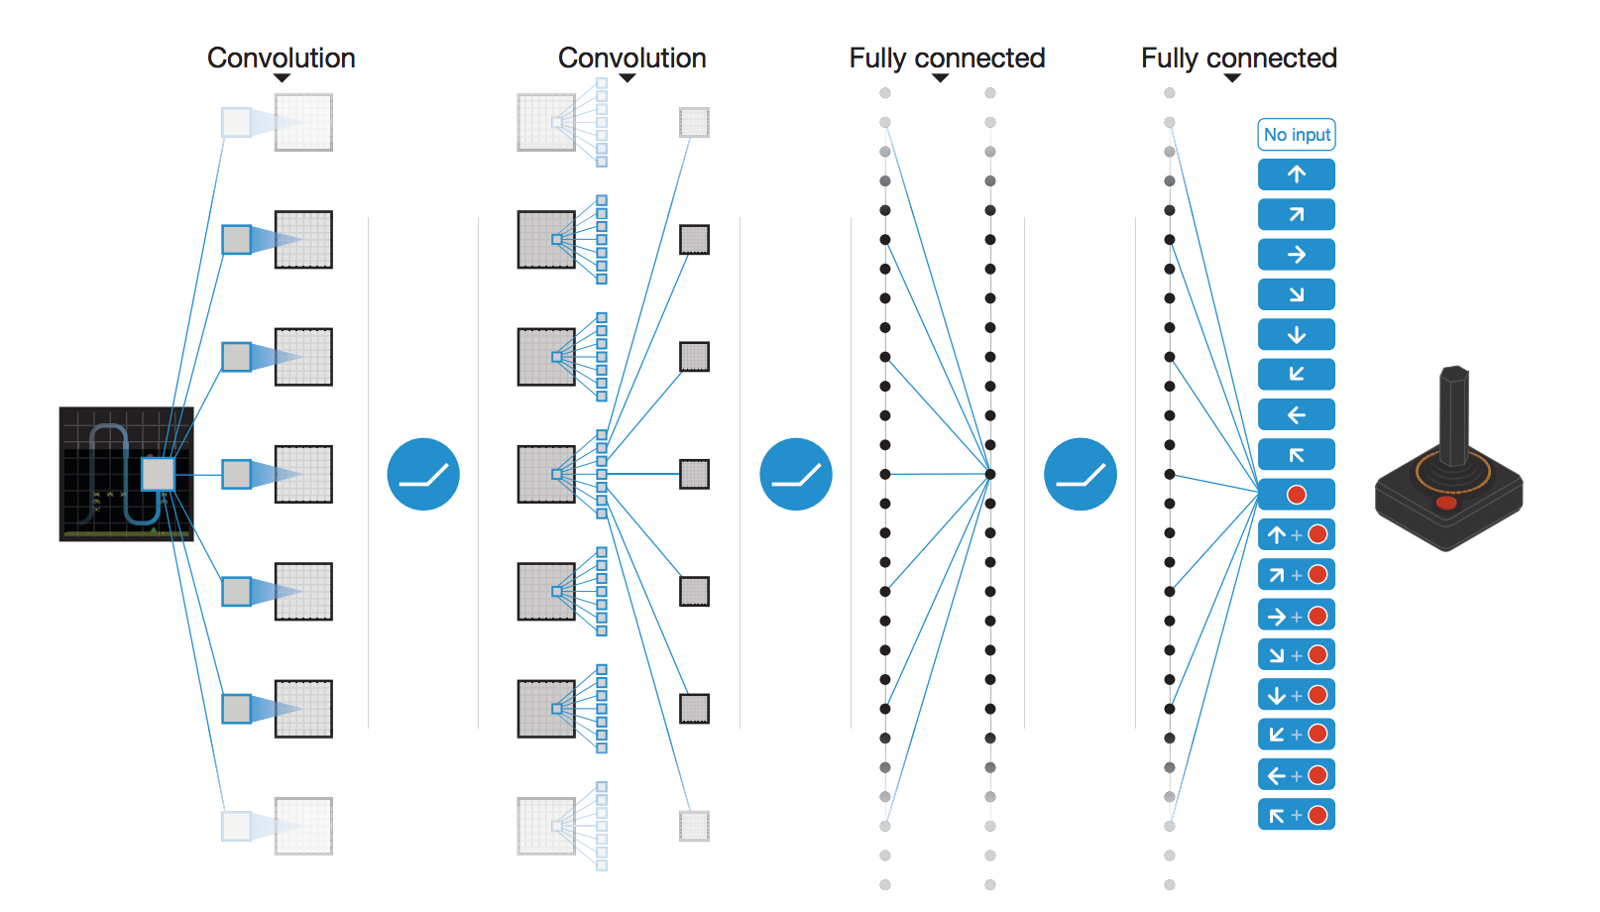
\includegraphics[width=0.9\linewidth]{fig/dqn1.png}
  \caption{\textbf{Goole团队DQN网络}}
  \label{fig:3-5}
\end{figure}

在Goole团队之前,也有研究人员使用神经网络近似Q值函数,但效果并不理想,DQN算法得以成功的具体细节如下所示:
\begin{enumerate}
  \item DQN利用CNN逼近Qlearning的$q(s,a)$即动作值函数
  \item DQN使用了经验回放机制(Experience Replay)训练智能体,经验回放机制是DQN算法获得成功的主要原因之一,DQN在于环境的迭代
   之中,前一个状态与后一个状态具有高度相关性,而神经网络要求训练数据彼此不相关,经验回放机制类似于 人类海马体的记忆原理,
   在算法中的具体体现为记录智能体与环境迭代的数据,记录数据达到一定数目后,之后就从记录的数据池中挑选数据,在喂入神经网络以打破数据之间的相关性。
  \item DQN设置双层神经网络,Qtarget和当前Q网络。两者结构相同,Qtarget网络的参数是当前Q网络参数延迟赋值得到的。在估计目标Q值时利用Qtarget网络进行估计,
  这种独特的设计减少了目标值与当前值之间的关联,是DQN获得成功的另一主要原因。
  
\end{enumerate}

DeepMind团队所用DQN算法的伪代码如下:\\
\begin{algorithm}[H]  
  \caption{使用经验回放的DQN}  
  \begin{algorithmic}
    \State 初始化 replay memory D 使用容量 N
    \State 初始化动作价值函数 $Q$ 使用随机的权重 
    \State {初始化target网络 $\hat{Q}$ 使用权重 $\theta ^{-}=\theta $ }
    \For{episode=1,M do}
    \State 初始化序列 $s_1={x_1}$ and 预处理序列 $\phi_1=\phi (s_1)$
    \For{t=1,T do}
    \State 使用可能性 $\epsilon$ 挑选随机动作 $a_t$
    \State 其他情况选择 $a_t=argmax_aQ(\phi(s_t),a;\theta)$
    \State 执行动作 $a_t$ 在仿真器并观察 $r_t$ 和图像 $x_{t+1}$
    \State 设置 $s_{t+1}=s_t,a_t,x_{t+1}$ 并且预处理$\phi_{t+1}=\phi(s_{t+1})$
    \State 存储过渡时期 $(\phi_t,a_t,r_t,\phi_{t+1})$ 在 D
    \State 在过渡时期存储库D中随机挑选样本 $(\phi_j,a_j,r_j,\phi_{j+1})$ 
    \State $$
    Set y_j=\begin{cases}
      r_j & if episode terminates at step j+1\\
      r_j+\gamma\max_{a^{'}}\hat{Q}(\phi_{j+1},a^{'};\theta^{-})&  otherwise
    \end{cases}
    $$
    \State 实施梯度下降法更新 $(y_j-Q(\phi_j,a_j;\theta))^2$其权重是网络参数 $\theta$
    \State Every C steps reset $\hat{Q}=Q$
    \EndFor 
    \EndFor
  \end{algorithmic}  
\end{algorithm}
\subsubsection{本文所用DQN算法框架}
本文所用DQN算法框架如图~\ref{fig:3-6}。
\begin{figure}[H]
  \centering
  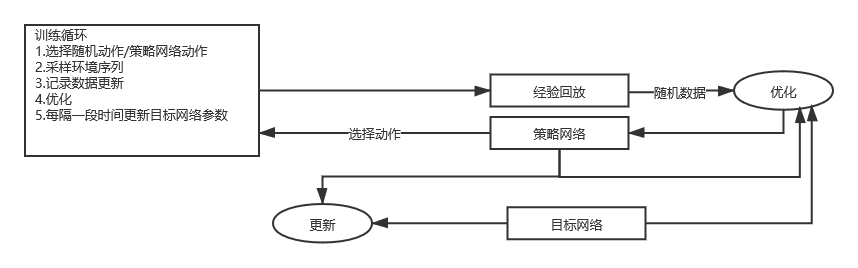
\includegraphics[width=0.7\linewidth]{fig/dqn_2.png}
  \caption{\textbf{本文所用DQN算法框架}}
  \label{fig:3-6}
\end{figure}

本文所用DQN依旧使用了CNN来 近似状态动作值函数,CNN由三个卷积层,三个BN(批处理层),一个全连接层构成。实验表明过多的神经网络层数并不能带来性能的提升,
这与强化学习探索和发现机制有关。本文的DQN网络使用Carla语义相机图片作为输入,输出为离散化的汽车控制指令,以实现一种端到端的决策模块。训练过程中也使用了Goole团队的训练技巧,包括建立双层网络,使用经验回放池,此外还对数据进行了预处理以加快训练,防止过拟合。
伪代码如下:\\
\begin{algorithm}[H]  
  \caption{DQN车道保持}  
  \begin{algorithmic}[1] 
    \Require CARLA语义相机R通道图片
    \Ensure 
    \State 初始化记忆矩阵D,初始化Q-target网络参数$w^{-}$和当前网络参数$w$
    \For{episde=1,M do}
    \State CARLA环境初始化,初始化到起点
    \For{t=1,...$T_{max}$ do}
    \State 采取上文提到的$\epsilon$贪心策略采取行动,记录$(s,a,r,s^{'})$于D
    \State 从记忆矩阵取出一批样本
    \State 用Q-target网络计算:$y=r+\gamma\max_{a^{'}}Q(s^{'},a^{'};w^{-})$
    \State 用$I=(r+\gamma\max_{a^{'}}Q(s^{'},a^{'};w^{-})-Q(s,a:w))^2$来提升参数
    \State 每隔N步将参数$w$赋值给$w^{-}$

    \EndFor
    \EndFor
     
  \end{algorithmic}  
\end{algorithm}
\subsection{本章小结}
本章介绍了强化学习和深度学习相关知识,具体介绍了本文所用的路径规划算法和车道保持算法。具体为使用Q学习和SARSA算法来进行路径规划,
并对上述方法的奖励函数进行了特别的设计,以满足用户不同的需求。除了路径规划之外,本文还将深度强化学习中的DQN算法用到车道保持任务中,仅使用Carla语义
相机输出的图片,做到车辆沿着车道行驶,避开了复杂的人工规则设计,具有一定实际价值。